\chapter{disturbing the vacuum: Casimir effect}
\begin{itemize}
	\item 考虑一个沿 $x^1$ 方向满足 periodic b.c. 的空间, 在垂直于 $x^1$ 方向有两个 plates, s.t. 在 plates 上 $\phi(x) = 0$, 如下图,
	
	\begin{figure}[H]
		\centering
		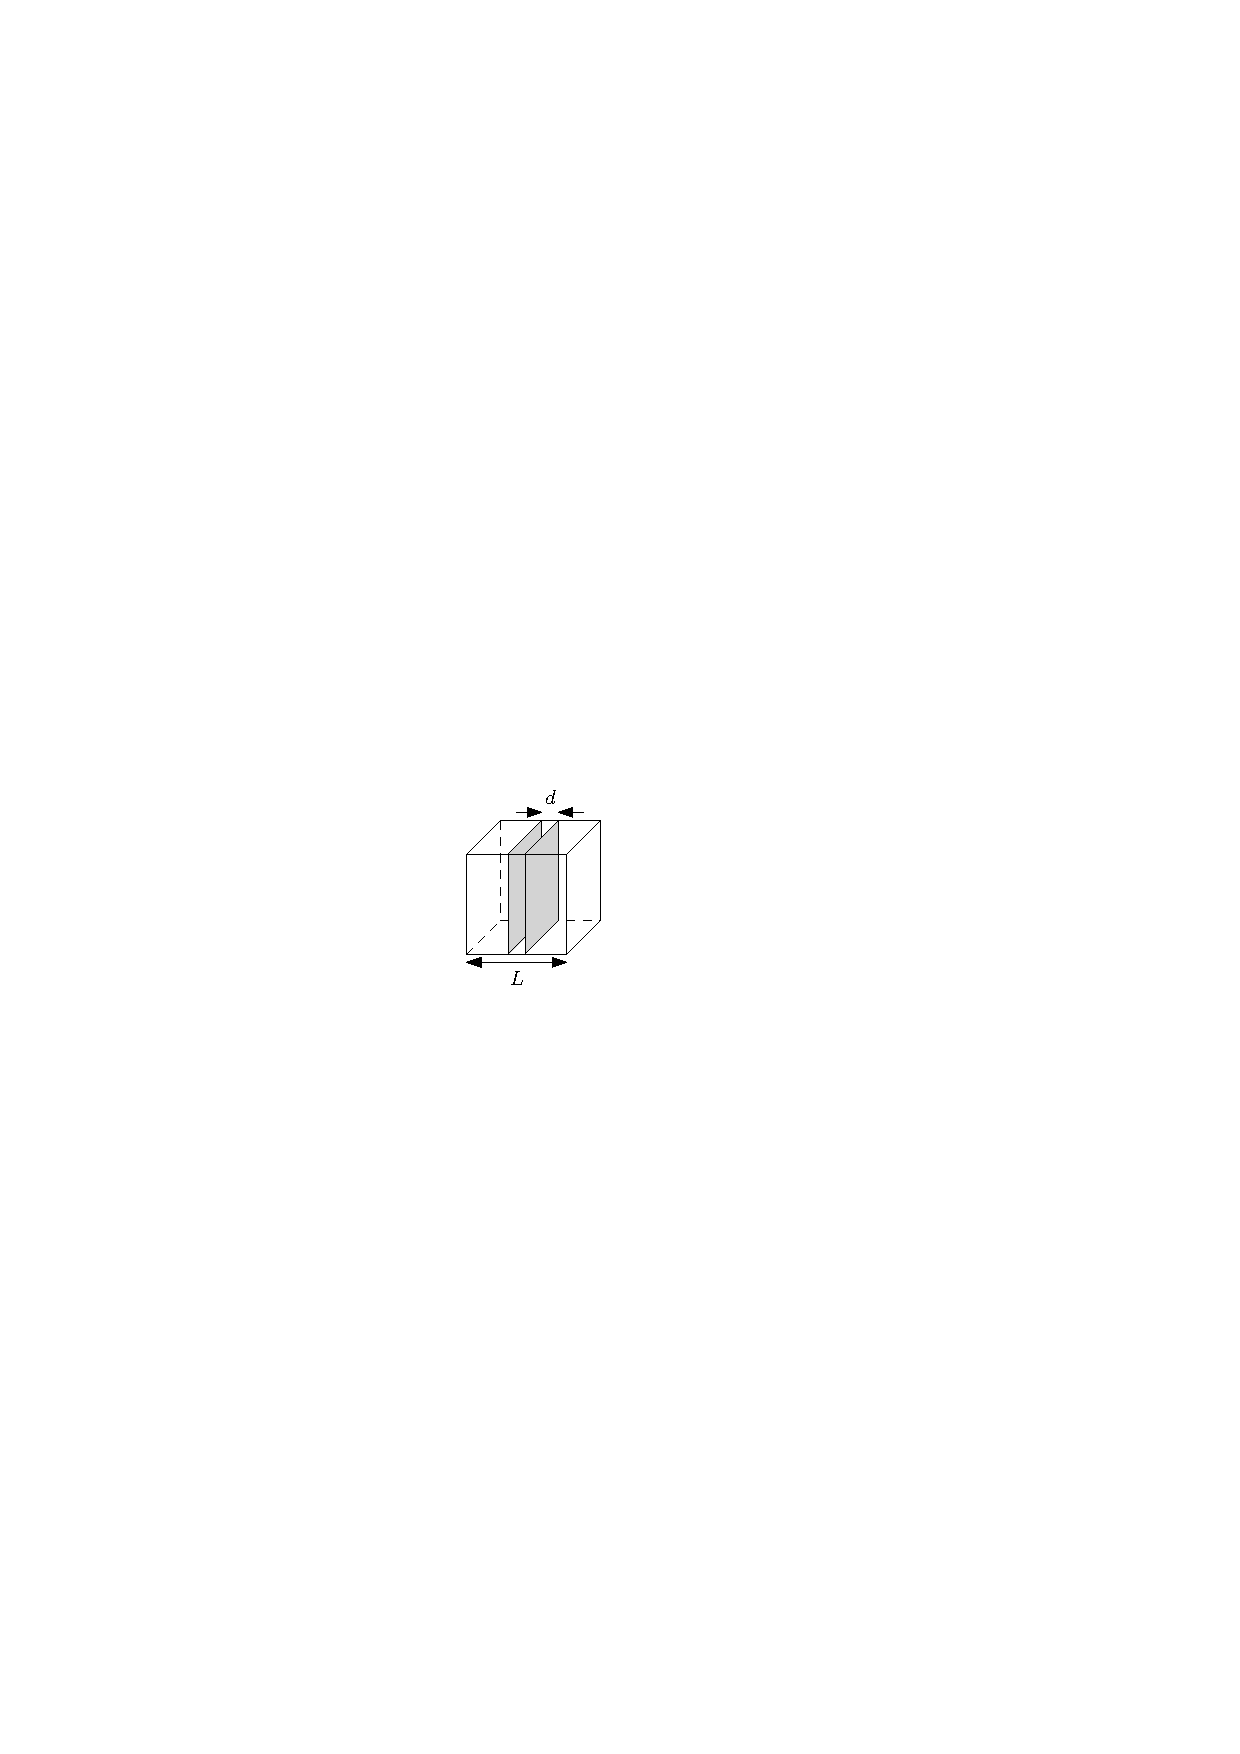
\includegraphics[scale=1]{figures/Casimir effect.pdf}
		\caption{Casimir effect}
	\end{figure}
	
	\item 平板内外, 标量场的波矢的取值为,
	\begin{equation}
		\begin{dcases}
			(n \frac{\pi}{d}, k_2, k_3) & \text{平板内} \\
			(n \frac{\pi}{L - d}, k_2, k_3) & \text{平板外}
		\end{dcases}
	\end{equation}
	其中 $n \in \mathbb{Z}^+$.
	
	\item 因此, 代入真空能公式 \eqref{4.1.15}, 平板内的能量为,
	\begin{equation}
		\frac{E(d)}{A} = \sum_{n = 1}^\infty \int \frac{dk_2 dk_3}{(2 \pi)^2} \frac{1}{2} \sqrt{\Big( n \frac{\pi}{d} \Big)^2 + k_2^2 + k_3^2}
	\end{equation}
	而总能量为 $E = E(d) + E(L - d)$.
	
	\noindent\rule[0.5ex]{\linewidth}{0.5pt} % horizontal line
	
	\item 为解决能量发散的问题, 引入 ultra-violet (UV) cut-off,
	\begin{equation}
		\frac{E(d)}{A} = \sum_{n = 1}^\infty \int \frac{dk_2 dk_3}{(2 \pi)^2} \frac{1}{2} \sqrt{\Big( n \frac{\pi}{d} \Big)^2 + k_2^2 + k_3^2} \, e^{- a \sqrt{(n \frac{\pi}{d})^2 + k_2^2 + k_3^2}}
	\end{equation}
	for some $a \ll d$.
	
	\item 为了简化问题, 考虑 $d = 1 + 1$ 的情况,
	\begin{equation}
		E_{1 + 1}(d) = \frac{\pi}{2 d} \sum_{n = 1}^\infty n e^{- \frac{a \pi}{d} n} = \frac{\pi}{2 d} \frac{e^{\frac{a \pi}{d}}}{(e^{\frac{a \pi}{d}} - 1)^2} = \frac{d}{2 \pi a^2} - \frac{\pi}{24 d} + O(a^2)
	\end{equation}
	因此,
	\begin{equation}
		E_{1 + 1} = E_{1 + 1}(d) + E_{1 + 1}(L - d) = \frac{L}{2 \pi a^2} - \frac{\pi}{24} \Big( \frac{1}{d} + \frac{1}{L - d} \Big) + O(a^2)
	\end{equation}
	得到 Casimir force,
	\begin{equation}
		F_{1 + 1} = - \frac{\partial E_{1 + 1}}{\partial d} = - \frac{\pi}{24} \Big( \frac{1}{d^2} - \frac{1}{(L - d)^2} \Big) + O(a^2) \overset{L \rightarrow \infty, a \rightarrow 0}{=} - \frac{\pi}{24 d^2}
	\end{equation}
	
	\item 问题中, $a$ 引入了 UV cut-off, $L$ 引入了 infrared cut-off.
\end{itemize}
